\documentclass{article}
\usepackage{graphicx}
\usepackage{tikz}
\usepackage{caption}
\usetikzlibrary{arrows.meta, positioning}
\usepackage{hyperref}
\usepackage{subcaption}
\usepackage[margin=1in]{geometry}
\usepackage{url}
\usepackage[colorlinks=true,citecolor=blue,urlcolor=blue]{hyperref}

\title{Technical Communication - Lab 3}
\author{UTKARSH KUMAR 23114101}
\date{February 2026}

\begin{document}

\maketitle

\begin{enumerate}
    \item 
    

In Figures \ref{fig:shift-register} and \ref{fig:checkerboard}, we show how to add images in \LaTeX{} with TikZ. The figures are taken from \cite{EME22}.

\begin{figure}[ht]
\centering

\resizebox{0.4\textwidth}{!}{%
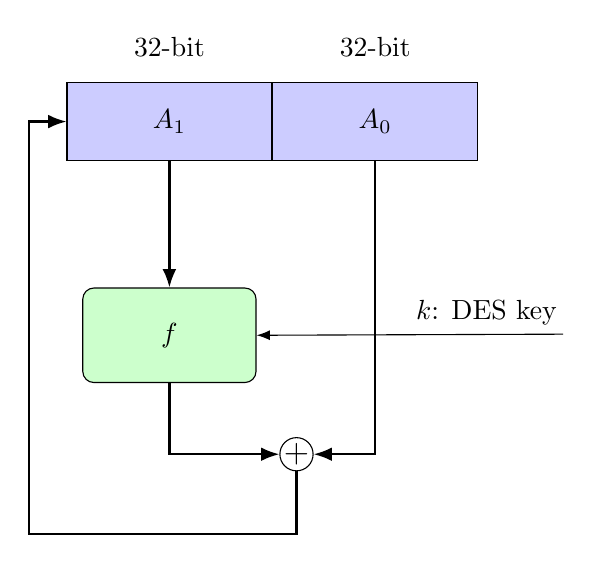
\begin{tikzpicture}[
    >=Latex,
    block/.style={
        draw,
        rectangle,
        minimum height=1cm,
        minimum width=2.6cm,
        fill=blue!20
    },
    func/.style={
        draw,
        rectangle,
        rounded corners,
        minimum height=1.2cm,
        minimum width=2.2cm,
        fill=green!20
    },
    arrow/.style={->, thick}
]

\node[block] (A1) {$A_1$};
\node[block, right=0pt of A1] (A0) {$A_0$};
\node[above=2mm of A1] {32-bit};
\node[above=2mm of A0] {32-bit};
\node[func, below=1.6cm of A1] (f) {$f$};
\node [draw, circle, inner sep=0pt, below=3.5cm of A0,xshift=-1cm] (xor) {\large $+$};

\draw[arrow] (A1.south) -- (f.north);
\draw[arrow] (A0.south) -- ++(0,0) |- (xor.east);
\draw[arrow] (f.south) -- ++(0,0) |- (xor.west);
\draw[arrow] (xor.south) -- ++(0,-0.8) -| ++(-3.4,0) |- (A1.west);
\draw [->] (5,-2.7) -- node[above,pos=0.25] {$k$: DES key} (f.east);

\end{tikzpicture}%
}

\caption{A diagram of word-based feedback shift register}
\label{fig:shift-register}
\end{figure}

\begin{figure}[ht]
\centering
\resizebox{0.4\textwidth}{!}{%
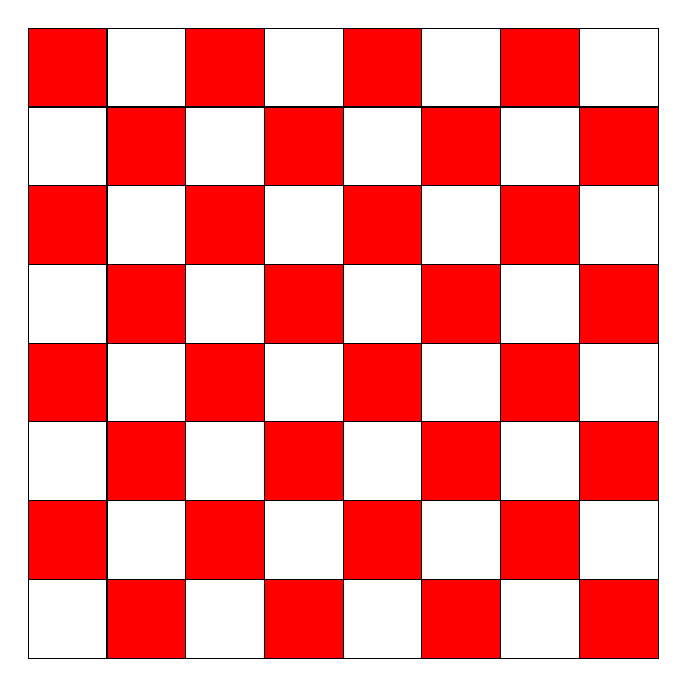
\begin{tikzpicture}
\foreach \x in {0,...,7} {
  \foreach \y in {0,...,7} {
    \pgfmathparse{mod(\x+\y,2)==0 ? "white" : "red"}
    \edef\colorname{\pgfmathresult}
    \filldraw[fill=\colorname, draw=black] (\x,\y) rectangle ++(1,1);
  }
}
\end{tikzpicture}%
}
\caption{A diagram of checkerboard}
\label{fig:checkerboard}
\end{figure}

\item 

In Figure \ref{fig:side-by-side}, we show how to add two figures side by side. In Figure \ref{fig:subfig}, we show how to use the subfigure environment. The subfigures are shown in Figures \ref{shift_sub} and
\ref{fig:check_sub} and taken from \cite[Section~1]{HDRM23}.

\begin{figure}[ht]
\centering

\resizebox{0.45\textwidth}{!}{%
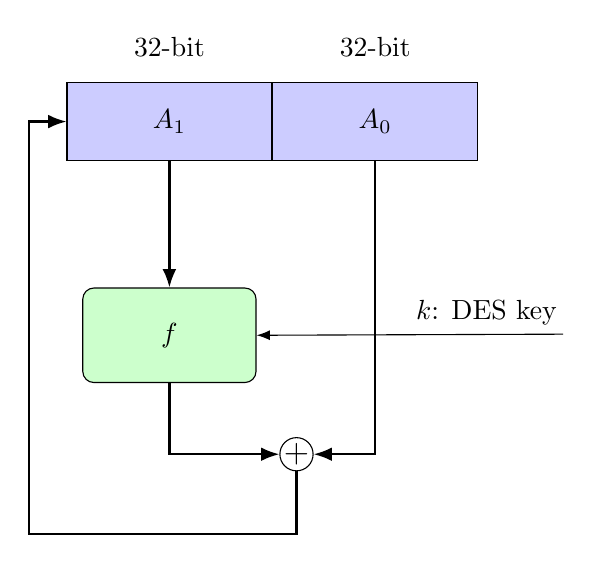
\begin{tikzpicture}[
    >=Latex,
    block/.style={
        draw,
        rectangle,
        minimum height=1cm,
        minimum width=2.6cm,
        fill=blue!20
    },
    func/.style={
        draw,
        rectangle,
        rounded corners,
        minimum height=1.2cm,
        minimum width=2.2cm,
        fill=green!20
    },
    arrow/.style={->, thick}
]

\node[block] (A1) {$A_1$};
\node[block, right=0pt of A1] (A0) {$A_0$};
\node[above=2mm of A1] {32-bit};
\node[above=2mm of A0] {32-bit};
\node[func, below=1.6cm of A1] (f) {$f$};
\node [draw, circle, inner sep=0pt, below=3.5cm of A0,xshift=-1cm] (xor) {\large $+$};

\draw[arrow] (A1.south) -- (f.north);
\draw[arrow] (A0.south) |- (xor.east);
\draw[arrow] (f.south) |- (xor.west);
\draw[arrow] (xor.south) -- ++(0,-0.8) -| ++(-3.4,0) |- (A1.west);
\draw [->] (5,-2.7) -- node[above,pos=0.25] {$k$: DES key} (f.east);

\end{tikzpicture}%
}
\hfill
\resizebox{0.45\textwidth}{!}{%
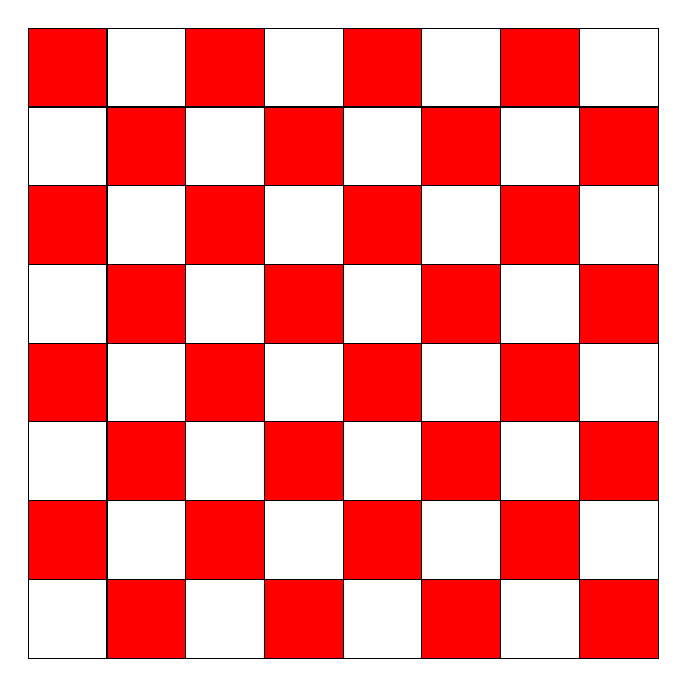
\begin{tikzpicture}
\foreach \x in {0,...,7} {
  \foreach \y in {0,...,7} {
    \pgfmathparse{mod(\x+\y,2)==0 ? "white" : "red"}
    \edef\colorname{\pgfmathresult}
    \filldraw[fill=\colorname, draw=black] (\x,\y) rectangle ++(1,1);
  }
}
\end{tikzpicture}%
}

\caption{Putting figures side by side}
\label{fig:side-by-side}
\end{figure}


\begin{figure}[ht]
\centering

\begin{subfigure}{0.45\textwidth}
\centering
\resizebox{\textwidth}{!}{%
% shift
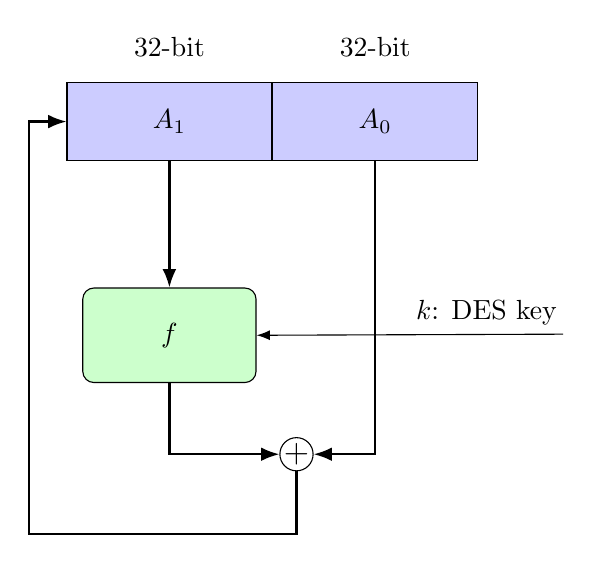
\begin{tikzpicture}[
    >=Latex,
    block/.style={
        draw,
        rectangle,
        minimum height=1cm,
        minimum width=2.6cm,
        fill=blue!20
    },
    func/.style={
        draw,
        rectangle,
        rounded corners,
        minimum height=1.2cm,
        minimum width=2.2cm,
        fill=green!20
    },
    arrow/.style={->, thick}
]

\node[block] (A1) {$A_1$};
\node[block, right=0pt of A1] (A0) {$A_0$};
\node[above=2mm of A1] {32-bit};
\node[above=2mm of A0] {32-bit};
\node[func, below=1.6cm of A1] (f) {$f$};
\node [draw, circle, inner sep=0pt, below=3.5cm of A0,xshift=-1cm] (xor) {\large $+$};

\draw[arrow] (A1.south) -- (f.north);
\draw[arrow] (A0.south) |- (xor.east);
\draw[arrow] (f.south) |- (xor.west);
\draw[arrow] (xor.south) -- ++(0,-0.8) -| ++(-3.4,0) |- (A1.west);
\draw [->] (5,-2.7) -- node[above,pos=0.25] {$k$: DES key} (f.east);

\end{tikzpicture}%
}
\caption{Shift register}
\label{shift_sub}
\end{subfigure}
\hfill
\begin{subfigure}{0.45\textwidth}
\centering
\resizebox{\textwidth}{!}{%
% check
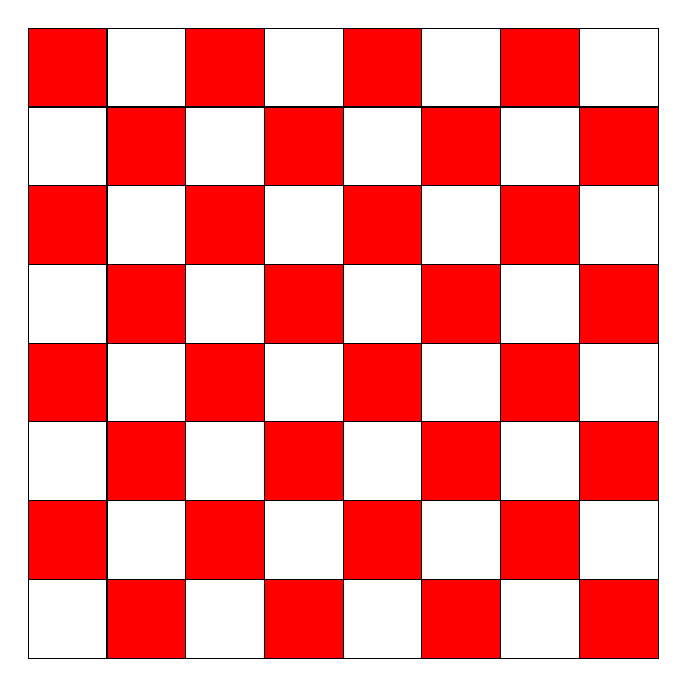
\begin{tikzpicture}
\foreach \x in {0,...,7} {
  \foreach \y in {0,...,7} {
    \pgfmathparse{mod(\x+\y,2)==0 ? "white" : "red"}
    \edef\colorname{\pgfmathresult}
    \filldraw[fill=\colorname, draw=black] (\x,\y) rectangle ++(1,1);
  }
}
\end{tikzpicture}%
}
\caption{Checkerboard}
\label{fig:check_sub}
\end{subfigure}

\caption{Subfigure environment}
\label{fig:subfig}
\end{figure}
\clearpage
\newpage
\item In the following we show how to use the minipage environment and add images in the same environment as shown in Figures \ref{fig:shift_mini} and \ref{fig:check_mini}. The resources are taken from \cite{Ind26}.

\begin{figure}[ht]
\centering

% shift
\begin{minipage}[t]{0.45\textwidth}
\textbf{Groups}

\vspace{4pt}

The ubiquitous student groups are what set IIT Roorkee apart
from the other technical institutes in India. Here do the like-minded
gather to work together toward a certain goal — be it getting out
a magazine on time, or putting together a one-hour concert, or making
a trip to a nearby village for social work. From togetherness comes
success and this feature of life here certainly adds spice to the lives
of the students.

\vspace{8pt}

\centering
\resizebox{0.9\linewidth}{!}{%
  % shift
  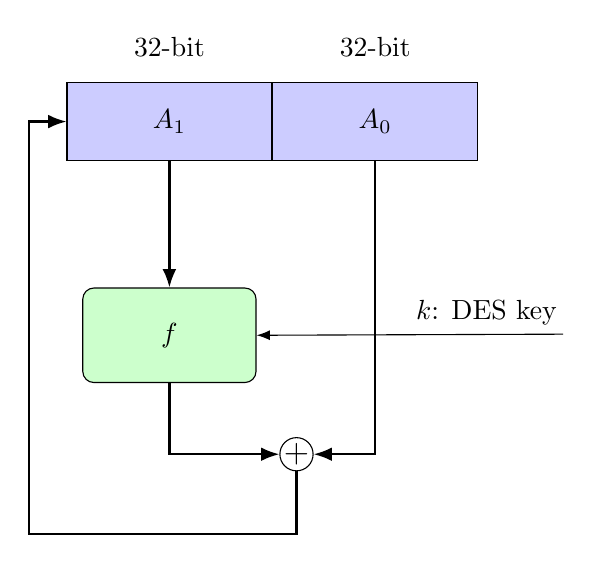
\begin{tikzpicture}[
    >=Latex,
    block/.style={
        draw,
        rectangle,
        minimum height=1cm,
        minimum width=2.6cm,
        fill=blue!20
    },
    func/.style={
        draw,
        rectangle,
        rounded corners,
        minimum height=1.2cm,
        minimum width=2.2cm,
        fill=green!20
    },
    arrow/.style={->, thick}
]

\node[block] (A1) {$A_1$};
\node[block, right=0pt of A1] (A0) {$A_0$};
\node[above=2mm of A1] {32-bit};
\node[above=2mm of A0] {32-bit};
\node[func, below=1.6cm of A1] (f) {$f$};
\node [draw, circle, inner sep=0pt, below=3.5cm of A0,xshift=-1cm] (xor) {\large $+$};

\draw[arrow] (A1.south) -- (f.north);
\draw[arrow] (A0.south) |- (xor.east);
\draw[arrow] (f.south) |- (xor.west);
\draw[arrow] (xor.south) -- ++(0,-0.8) -| ++(-3.4,0) |- (A1.west);
\draw [->] (5,-2.7) -- node[above,pos=0.25] {$k$: DES key} (f.east);

\end{tikzpicture}%
}

\captionof{figure}{Shift register within Minipage}
\label{fig:shift_mini}
\end{minipage}
\hfill
% check
\begin{minipage}[t]{0.45\textwidth}
\textbf{Fitness}

\vspace{4pt}

Fit India Mission encourages people to become part of Fit India
Movement by inculcating at least 30–60 minutes of physical activities
in their day-to-day lives. The mission of the Movement is to bring about
behavioral changes and move towards a more physically active lifestyle.

\vspace{8pt}

\centering
\resizebox{0.9\linewidth}{!}{%
  % check
  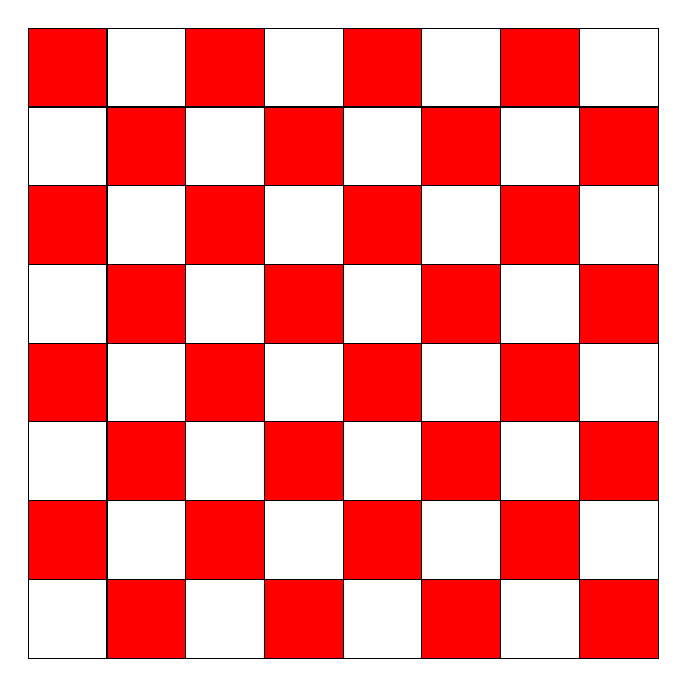
\begin{tikzpicture}
\foreach \x in {0,...,7} {
  \foreach \y in {0,...,7} {
    \pgfmathparse{mod(\x+\y,2)==0 ? "white" : "red"}
    \edef\colorname{\pgfmathresult}
    \filldraw[fill=\colorname, draw=black] (\x,\y) rectangle ++(1,1);
  }
}
\end{tikzpicture}%
}

\captionof{figure}{Checkerboard within Minipage}
\label{fig:check_mini}
\end{minipage}

\end{figure}


\item The references \cite{HDRM23,EME22,Ind26} are used in this lab.


\end{enumerate}

\bibliographystyle{alpha}
\bibliography{refs}

\end{document}
